%%%%%%%%%%%%%%%%%%%%%%%%%%%%%%%%%%%%%%%%%%%%%%%%%%%%%%%%%%%%%%%%%%%%%%%%%%%%%%%%
%2345678901234567890123456789012345678901234567890123456789012345678901234567890
%        1         2         3         4         5         6         7         8

\documentclass[letterpaper, 10 pt, conference]{ieeeconf}  % Comment this line out if you need a4paper

%\documentclass[a4paper, 10pt, conference]{ieeeconf}      % Use this line for a4 paper

\IEEEoverridecommandlockouts                              % This command is only needed if 
                                                          % you want to use the \thanks command

\overrideIEEEmargins                                      % Needed to meet printer requirements.

%In case you encounter the following error:
%Error 1010 The PDF file may be corrupt (unable to open PDF file) OR
%Error 1000 An error occurred while parsing a contents stream. Unable to analyze the PDF file.
%This is a known problem with pdfLaTeX conversion filter. The file cannot be opened with acrobat reader
%Please use one of the alternatives below to circumvent this error by uncommenting one or the other
%\pdfobjcompresslevel=0
%\pdfminorversion=4

% See the \addtolength command later in the file to balance the column lengths
% on the last page of the document

% The following packages can be found on http:\\www.ctan.org
\usepackage{graphics} % for pdf, bitmapped graphics files
\usepackage{epsfig} % for postscript graphics files
\usepackage{mathptmx} % assumes new font selection scheme installed
\usepackage{times} % assumes new font selection scheme installed
\usepackage{amsmath} % assumes amsmath package installed
\usepackage{amssymb}  % assumes amsmath package installed

\usepackage[brazilian]{babel}
\usepackage[utf8]{inputenc}
\usepackage[T1]{fontenc}
\DeclareUnicodeCharacter{0301}{\'{e}}

\title{\LARGE \bf
Entropy and Clustering Information\\
Applied to sEMG Classification.
}


\author{Luiz J. L. Barbosa$^{1}$, Otávio Nogueira$^{2}$, Vinícius de Oliveira Silva$^{2}$,\\Paulo V. P. Cotta$^{1}$, Fernando Vinícius Gonçalvez de Souza$^{1}$,\\Michael Douglas do Carmo de Araujo$^{2}$, Pedro Henrique Gonçalaves Inazawa$^{1}$,\\Alberto López-Delis$^{3}$ and Adson F. da Rocha$^{2}$% <-this % stops a space
\thanks{*This work was partially supported by CAPES and CNPq.}% <-this % stops a space
\thanks{$^{1}$Luiz Barbosa and Paulo V. P. Cotta, Fernando de Souza and Pedro Inazawa are with the Biomedical Engineering Program University of Braslia - Gama, Braslia, DF 70910-900, Brazil 
        {\tt\small contato@luizbarbosa.net}}%
\thanks{$^{2}$Otávio Nogueira, Vinı́cius de Oliveira Silva, Michael do Carmo and Adson Ferreira da Rocha are with the Department of Electrical Engineering University of Braslia, Braslia, DF 70910-900, Brazil adson@unb.br
        {\tt\small adson@unb.br}}%
\thanks{$^{3}$Alberto López-Delis with the Medical Biophysic Center: Santiago de Cuba, Santiago de Cuba, Cuba
        {\tt\small lopez.delis69@gmail.com}}%
}


\begin{document}



\maketitle
\thispagestyle{empty}
\pagestyle{empty}


%%%%%%%%%%%%%%%%%%%%%%%%%%%%%%%%%%%%%%%%%%%%%%%%%%%%%%%%%%%%%%%%%%%%
\begin{abstract}

The EMG signal is very difficult to classify due to the stochastic complexity of its characteristics. A way to reduce the complexity of a signal is to use clusters to resize them to a smaller space and then perform the classification. A classification improvement was verified by clustering the electromyographic signal and comparing it with the possible movements that can be performed. In this study, the Agglomerative Hierarchical Clustering was used. The basic
idea is to give prior information to the final classifier so the posterior classification has fewer classes, diminishing his complexity. Through the methodology applied in this article, an accuracy of more than 90\% was achieved by using a time window of only 10 ms in a signal sampled at 2000 Hz. Experimentation confirms that the methods presented in this paper are competitive in the state of the art.

%\newline
%
%\indent \textit{Clinical relevance}— This is a brief additional statement on why a this might be of interest to %practicing clinicians. Example: This establishes the anesthetic efficacy of 10\% intraosseous injections with %epinephrine to positively influence cardiovascular function.
\end{abstract}



%%%%%%%%%%%%%%%%%%%%%%%%%%%%%%%%%%%%%%%%%%%%%%%%%%%%%%%%%%%%%%%%%%%%%%%%%%%%%%%%
\section{INTRODUCTION}

The electromyographic (EMG) signal varies according to the posture, position, and force applied by the person that is
performing a muscle contraction. Therefore, to have perfect control of a prosthesis, extensive training with a myoelectric unit is required. However, as these prostheses have a high cost investment, it is often not possible to offer long-term training for their use. 

One of the difficulties regarding EMG signal processing for use in prosthesis control is the need for real-time processing. This creates the need for ever-smaller time windows that, in turn, have less signal information, which limits the amount of information that can be extracted from them. 

In the last few years, deep learning techniques have become increasingly used, but the more complex the applications are, the more complex the neural networks become. However, the more parameters the network has, the higher the chance of having over-fitting, which causes considerable deterioration to the network’s generalization capacity. Otherwise, if the neural network has few parameters, it will
probably not be able to represent the data accurately. Notably, the best way to achieve generalization is to seek a balance between training error and network complexity \cite{c1}, \cite{c2}.

In the tasks of biosignal classification, there are frequently too few biomedical signal samples to allow for the achievement of good results with deep learning \cite{c3}. Another problem associated with deep learning is the cost of training processing, which demands specific hardware and high computational cost due to the complexity of the current neural networks architectures \cite{c4}. This paper suggests extracting maximum signal information before signal classification as a method to reduce the system complexity and create redundancy for the classification and thereby managing to decrease the time window for the real-time processing of the signal. One of the steps of the algorithm proposed includes the development of a pipeline that extracts a priori information from the EMG signal by computing the current hand and forearm postures and the similarity of the EMG signals from the forearm.

As mentioned before, one way to ensure entropy reduction (information gain) is to obtain a priori information \cite{c5}. The starting position of the hand and forearm provide a great deal of information to the classifier as it restricts possible movement classes. For this purpose, a state machine \cite{c6} that counts the possible movements from the initial classes was created. This state machine reduced by just over three times the number of classes to classify, improving the classification of the system.

A second method used in this work for entropy reduction, was the classification of signals by similarity. Therefore, a Hierarchical Agglomerative clustering (HCA) technique was selected. In this technique, each data point is considered an individual cluster. At each iteration, using distance, a similar pair of clusters are merged as they move up the hierarchy, until there is a formation of one cluster or K clusters.

The proposed methodology led to a substantial decrease in the size of the temporal window used for sEMG signal processing. Besides, there was also an improvement in the generalization and processing speed due to the simplification of the model used for classification.

This paper is organized as follows: Section II shows a detailed explanation of the algorithms used. The results are listed in Section III, which also presents a detailed analysis of the experiment. Finally, there is a conclusion, where the results are summarized.

\section{METHODOLOGY}

\subsection{The Pipeline}

Initially, there is an estimation of the original positions of the hand and forearm. The possible movements are checked by analyzing the state machine; these two steps lead to a list of values associated with the neurons that are activated in the final layer of the classifier.

\begin{figure}[h]
    \begin{center}
	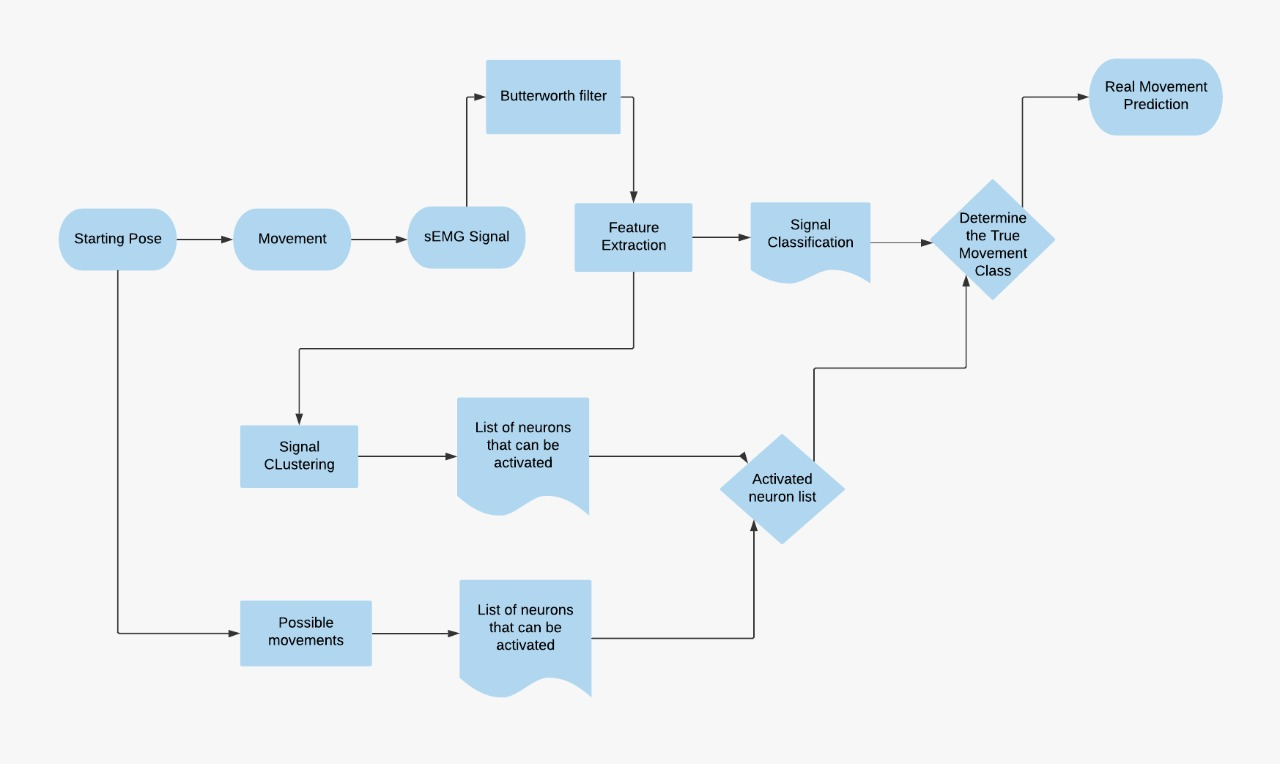
\includegraphics[width=.8\linewidth]{images/sMEG_Classification_Fluxogram.png}
	\end{center}
	\caption{Pipeline representation: the algorithm begins at a starting position; the sEMG signal is measured and pre-processed to help to determine the movement intention; with these two information pieces, the possible next movements are determined as well as the cluster to which the class belongs; finally, the algorithm yields the movement intention.} \label{fig_class_fluxo}
\end{figure}

The second step is processing the signal with the Butterworth filter, followed by the feature extraction and standardization of the data. Furthermore, a reduced space transform created by the Neighbourhood Components Analysis (NCA) algorithm is applied, and the signal is ready for the classification and clustering algorithms. This transformation reduces the vector of characteristics from 36 to 25 dimensions.

The third step for signal classification is to find the group to which the analyzed window belongs. The HAC clustering
algorithm will provide a new list of activated neurons in the classifier. In the HCA algorithm, each observation starts in its cluster, and the algorithm merges pairs of clusters when one moves up the hierarchy. The intersection between the state machine-generated list and the cluster generates the final list of neurons that can be activated.

The last step is the signal classification by the MLP and the multiplication of the result by the list generated in the previous step. The image below shows the value of neurons before and after applying the list of neurons to be used.

\subsection{Feature extraction}

In order to reduce signal noise, the first step in extracting features was to use a sixth-order bandpass Butterworth filter, 80-450Hz. Additionally, a time window for sampling the signal is selected. In this study, the sampling frequency of the sEMG was 2000 Hz, with a 0.01s window (i.e., ten samples per window).
This stage was subdivided into two steps:
\begin{enumerate}
    \item \textbf{Selection of characteristics:} to extract information from the signal four frequency domain features were used \cite{c9}:
        \begin{itemize}
            \item Spectral Moment;
            \item Waveform Length (accumulative changes in the length);
            \item Mean;
            \item Median;
        \end{itemize}
   \item \textbf{Dimensional reduction:} NCA~\cite{c10} allowed for the dimensional reduction by helping to select the most significant features of the signal. NCA is a supervised learning algorithm for distance metric learning. It learns a linear transformation (of input data) that maximizes, in the transformed space, the average leave-one-out classification performance. 
\end{enumerate}

\subsection{Signal Information}

To extract the maximum information of the signal the processes were divided into two steps:

\begin{enumerate}
	\item Signal Clustering: Agglomerative Hierarchical Clustering (HCA) clusterized the signal into three groups according to the similarity of the features. The HAC algorithm recursively merges the pair of clusters that minimally increases a given linkage distance~\cite{c11,c12};
	\item Comparison with possible movements: after the creation of the cluster, the algorithm compares movements classes with the possible movements for a given position, and the classes are extracted through a process called Decision Tree or State Machine~\cite{c13}.
\end{enumerate}

\subsection{Classifier Algorithm}
A simple multi-layer perceptron (MLP), with three layers, was used to classify the signal. The first layer was composed of 25 neurons, the middle layer by 52 neurons and the last by 26 neurons. In the first two layers, the linear rectifier was used as activation function. The last layer had a softmax function helping in the classification process. A dropout function (20\%), placed between the MLP layers, reduce the chance of over-fitting.The MLP was chosen because of its inherent capacity of simultaneous classification~\cite{c5}.

\begin{figure}[h]
    \begin{center}
	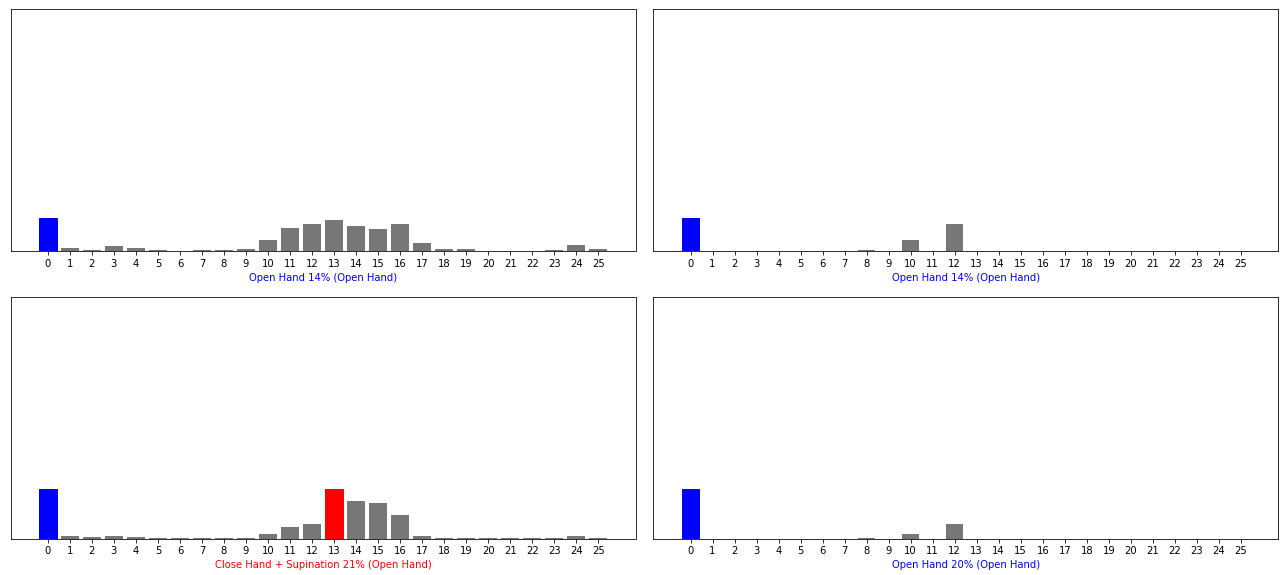
\includegraphics[width=.8\linewidth]{images/output2.png}
	\end{center}
	\caption{Output of the values of the MLP neurons of the last layer. The blue color mean the right classification and the red the wrong classification. The left figure is the output of the MLP and the right figure is the result with the possible classes only.} \label{final_classification}
\end{figure}

\subsection{Database}

The "6mov8chUFS" database~\cite{c7} consists of 17 patients, with six individual movement classes selected, such as opening and closing the hand, flexion and extension of the wrist, and prono-supination of the hand, forming 27 possible movements. The signal was measured as follows: 3 seconds of contraction time with 3 seconds for relaxation between each repetition, repetitions of each movement. 8 bipolar electrodes (disposable Ag / AgCl), 1 cm of electrode diameter, 2 cm of inter-electrode distance for the bipolar Electrodes were equally spaced around the proximal third of the forearm.

The algorithm was tested with the "6mov8chFUS" database, made available by BioPatRec platform~\cite{c8}. Also, with the help of the BioPatRec platform, an analysis was made using seventeen characteristics. With the use of NCA the four best characteristics for the execution of the algorithm were selected. The number of features was chosen to take into account the speed of the information processing, which needed to be as fast as possible to create the most natural movement possible.

\subsection{Movement Classes}

The movement classes used in the "6mov8chUFS" database are listed as follows:

\begin{enumerate}
    \item Open Hand
    \item Close Hand
    \item Flex Hand
    \item Extend Hand
    \item Pronation
    \item Supination
    \item Open Hand + Flex Hand
    \item Close Hand + Flex Hand
    \item Open Hand + Extend Hand
    \item Close Hand + Extend Hand
    \item Open Hand + Pronation
    \item Close Hand + Pronation
    \item Open Hand + Supination
    \item Close Hand + Supination
    \item Flex Hand + Pronation
    \item Extend Hand + Pronation
    \item Flex Hand + Supination
    \item Extend Hand + Supination
    \item Open Hand + Flex Hand + Pronation
    \item Close Hand + Flex Hand + Pronation
    \item Open Hand + Flex Hand + Supination
    \item Close Hand + Flex Hand + Supination
    \item Open Hand + Extend Hand + Pronation
    \item Close Hand + Extend Hand + Pronation
    \item Open Hand + Extend Hand + Supination
    \item Close Hand + Extend Hand + Supination
\end{enumerate}

\section{Results}

A recent study~\cite{c14} shows the impact of the temporal window size on the EMG signal classification error. According to this study, with very small windows, (on average less than 200 ms), the classification error increases as the total information in the window decreases. This feature makes real-time processing very difficult, since it requires small temporal windows. Moreover, in 2011 Peerdeman~\cite{c15} found that the processing window needs to have less than 300 ms, or the delay becomes unacceptable to the user.

The proposals studied in this article aim to reduce this limit from 200 to 300 milliseconds by creating mechanisms that allow for using smaller windows. Through these smalltime windows, it is possible to perform real-time processing.

Because of the small size (10ms) of the window, the MLP did not achieve a good signal classification, but the selection of which neurons are active for the classification, significantly increased the accuracy. Figure 2 shows the difference in the classification using only the possible classes.

For the clustering algorithm, three data clusters were created and evaluated using a KNN (k = 3). This KNN achieved 97\% accuracy by classifying the groups created, as seen in figure \ref{fig_sMEG_Clustering}.

\begin{figure}[h]
	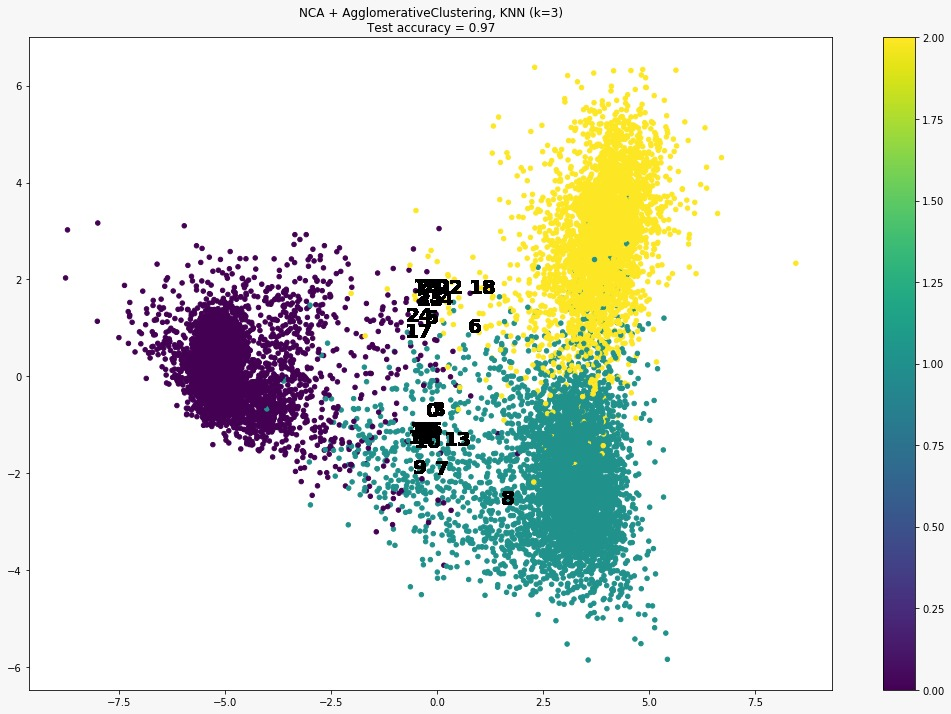
\includegraphics[width=\linewidth]{images/sMEG_Clustering.png}
	\caption {sMEG Clustering the classes by the similarity in the features extracted. After the extraction of twenty-five dimensions, the two more representative dimensions among them were used to generate the plot. A KNN was used to validate the cluster.} \label{fig_sMEG_Clustering}
\end{figure}

Table \ref{acc_std} shows the accuracy and standard deviation of MLP used in this article. The left side shows the results for the full MLP, and the right colulmn shows the, the results after the application of the pipeline shown in figure \ref{fig_class_fluxo}.

\begin{table}[h]
\caption{Accuracy and Standard Deviation Comparison}
\label{acc_std}
    \begin{center}
        \begin{tabular}{|c||c||c|}
        \hline
            & Ful MLP Output & with Selectd Neurouns \\ \hline
        Acc & 0.382          & 0.913                 \\ \hline
        Std & 0.013          & 0.011                 \\ \hline
        \end{tabular}
    \end{center}
\end{table}

Although the standard deviation remained relatively unchanged, the improvement in accuracy was immense. This achievement can be reached by excluding very close classes, such as closing and flexing the hand or opening and flexing the hand, where misclassifications generally occur.

\section{Conclusion}

In this thesis, two methods were used to obtain a priori information and thus reduce signal entropy before classification. New methods can bring even more significant improvement to the system. By providing a priori information for signal classification interactively, the number of possible classes for signal classification dramatically decreases. Creating less complex validation steps also increased accuracy while allowing window size reduction. We believe that the techniques presented here only scratch the surface of the applications where information entropy can and should be used.

The main idea of this study was to create a network that is simple and, through a small number of bits, can generalize the data better than a more complex network. Therefore, it is imperative to provide tools that simplify or provide data information. Besides, a simple neural network will have faster processing time and use less energy, being cheaper to train and more efficient to apply. Thus, providing tools that simplify or provide data information is critical. Furthermore, more studies to account for the trade-off between the number of steps and the processing time of the pipeline is needed.

\addtolength{\textheight}{-12cm}   % This command serves to balance the column lengths
                                  % on the last page of the document manually. It shortens
                                  % the textheight of the last page by a suitable amount.
                                  % This command does not take effect until the next page
                                  % so it should come on the page before the last. Make
                                  % sure that you do not shorten the textheight too much.

%%%%%%%%%%%%%%%%%%%%%%%%%%%%%%%%%%%%%%%%%%%%%%%%%%%%%%%%%%%%%%%%%%%%%%%%%%%%%%%%



%%%%%%%%%%%%%%%%%%%%%%%%%%%%%%%%%%%%%%%%%%%%%%%%%%%%%%%%%%%%%%%%%%%%%%%%%%%%%%%%



%%%%%%%%%%%%%%%%%%%%%%%%%%%%%%%%%%%%%%%%%%%%%%%%%%%%%%%%%%%%%%%%%%%%%%%%%%%%%%%%
\section*{APPENDIX}

Appendixes should appear before the acknowledgment.

\section*{ACKNOWLEDGMENT}

The preferred spelling of the word ÒacknowledgmentÓ in America is without an ÒeÓ after the ÒgÓ. Avoid the stilted expression, ÒOne of us (R. B. G.) thanks . . .Ó  Instead, try ÒR. B. G. thanksÓ. Put sponsor acknowledgments in the unnumbered footnote on the first page.



%%%%%%%%%%%%%%%%%%%%%%%%%%%%%%%%%%%%%%%%%%%%%%%%%%%%%%%%%%%%%%%%%%%%%%%%%%%%%%%%

References are important to the reader; therefore, each citation must be complete and correct. If at all possible, references should be commonly available publications.



\begin{thebibliography}{99}

\bibitem{c1} LeCun, Y., Denker, J. S., \& Solla, S. A. (1990). Optimal Brain Damage (Pruning). Advances in Neural Information Processing Systems, 598605.
\bibitem{c2}] Zhang, C., Recht, B., Bengio, S., Hardt, M., \& Vinyals, O. (2019). Understanding deep learning requires rethinking generalization. 5th International Conference on Learning Representations, ICLR 2017 - Conference Track Proceedings.
\bibitem{c3} Sarunas, J. R. \& A. K. J. (1991). Small Sample Size Effects in Statistical Pattern Recognition: Recommendations for Practiotioners.
\bibitem{c4} Zhang, C., Recht, B., Bengio, S., Hardt, M., \& Vinyals, O. (2019). Understanding deep learning requires rethinking generalization. 5th International Conference on Learning Representations, ICLR 2017 - Conference Track Proceedings.
\bibitem{c5} C.E. Shannon , vol. 27, pp. , July, October, ” ”. (1948). A Mathematical Theory of Communication. Bell System Tech- nical Journal, 27(April 1928), 379-423,623-656. Retrieved from http://math.harvard.edu/ctm/home/text/others/shannon/entropy/entropy.pdf
\bibitem{c6} Asghari Oskoei, M., \& Hu, H. (2007). Myoelectric control systems-A survey. Biomedical Signal Processing and Control. https://doi.org/10.1016/j.bspc.2007.07.009.
\bibitem{c7} Ortiz-catalan, M., Hkansson, B., \& Brnemark, R. (2014). Real-Time and Simultaneous Control of Arti fi cial Limbs Based on Pattern Recognition Algorithms. 22(4), 756764.
\bibitem{c8} Ortiz-Catalan, M., Brnemark, R., \& Hkansson, B. (2013). BioPatRec: A modular research platform for the control of artificial limbs based on pattern recognition algorithms. Source Code for Biology and Medicine. https://doi.org/10.1186/1751-0473-8-11.
\bibitem{c9} Jos, L., Barbosa, L., Roberto, P., Oliveira, F. De, Araujo, P. D., Ferreira, A., Lpez-delis, A. (2018). Simultaneous Myoelectric Pattern Recognition using BioPatRec Platform for Hand Prosthesis. XXVI Brazilian Congress on Biomedical Engineering, 869. https://doi.org/10.1007/978-981-13-2119-1
\bibitem{c10} Phinyomark A., Campbell E., Scheme E. (2020) Surface Electromyography (EMG) Signal Processing, Classification, and Practical Considerations. In: Naik G. (eds) Biomedical Signal Processing. Series in BioEngineering. Springer, Singapore
\bibitem{c11} Baek S, Hong Y, Choi S, et alElectrodiagnostic data-driven clustering identifies a prognostically different subgroup of patients with chronic inflammatory demyelinating polyneuropathyJournal of Neurology, Neurosurgery \& Psychiatry 2019;90:674-680.
\bibitem{c12} Y. Gloumakov, A. J. Spiers and A. M. Dollar, ”A Clustering Approach to Categorizing 7 Degree-of-Freedom Arm Motions during Activities of Daily Living,” 2019 International Conference on Robotics and Automation (ICRA), Montreal, QC, Canada, 2019, pp. 7214-7220. doi: 10.1109/ICRA.2019.8794421.
\bibitem{c13} Delisle-Rodriguez, D., Villa-Parra, A., Bastos-Filho, T., Lpez-Delis, A., Frizera-Neto, A., Krishnan, S., \& Rocon, E. (2017). Adaptive Spatial Filter Based on Similarity Indices to Preserve the Neural Information on EEG Signals during On-Line Processing. Sensors, 17(12), 2725. https://doi.org/10.3390/s17122725.
\bibitem{c14} Radhika Menon, Student Member, IEEE, Gaetano Di Caterina, Heba Lakany, Member, IEEE, Lykourgos Petropoulakis, Bernard A. Conway, John J. Soraghan, Senior Member, I. (n.d.). Study on interaction between temporal and spatial information in classification of EMG signals for myoelectric prostheses. https://doi.org/10.1109/TNSRE.2017.2687761.
\bibitem{c15} Peerdeman, B., Boere, D., Witteveen, H., Huis in ‘tVeld, R., Hermens, H., Stramigioli, S., Misra, S. (2011). Myoelectric forearm prostheses: State of the art from a user-centered perspective. The Journal of Rehabilitation Research and Development, 48(6), 719. https://doi.org/10.1682/JRRD.2010.08.0161.

\end{thebibliography}




\end{document}
